\documentclass[a4paper,10pt]{article}
\usepackage[margin=2.5cm, nohead]{geometry}
\usepackage{graphicx}
\usepackage{verbatim}
\newcommand{\Ardrone}{Ar Drone$^{\copyright}$ }

\title{Autonomous Flight With the \Ardrone}
\author{Maarten Inja \& Maarten de Waard\\\small 5872464 \& 5894883}

% The presentatie 

\begin{document}
\maketitle

\section{Introduction}

\subsection{The \Ardrone}
The \Ardrone is an over WiFi remote controlled quadrocopter that has several onboard sensors:
\begin{itemize}
	\item One vertical camera, pointing downwards
	\item One horizontal camera, pointing forward 
	\item Ultrasound altimeter, to measure the altitude
    \item 3 axis accelerometer (measures propellor acceleration)
    \item 2 axis gyrometer 
    \item 1 yaw precision gyrometer
\end{itemize}
Furthermore, it has an onboard computer system running Linux. 


\subsection{Our Goal}
Summer-IMAV 2011 Indoor competition, some sub-tasks of the exploration challenge:
\begin{itemize}
    \item Pick-up Object
    \item Exit Building
    \item Release Object
\end{itemize}


\section{Controlling the \Ardrone}
The \Ardrone has, like any other flying vehicle, the usual 3 critical flight dynamic parameters for the angles of rotation; pitch, yaw and roll (See figure 
\ref{pitchYawRoll}). In addition to these three parameters the \Ardrone has the \textit{gaz} parameter to control the upward or downward change. This allows
a pilot to increase or decrease the altitude directly. 

\begin{figure}[h!]
    \centering
        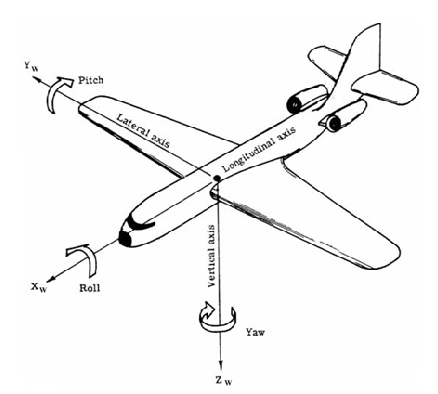
\includegraphics[scale=0.5]{pitchYawRoll.png}
    \caption{Movement directions for flying vehicles}
    \label{pitchYawRoll}
\end{figure}

\subsection{ROS And AT Commands}
ROS, or Robot Operating System, is an open-source, meta-operating system for your robot. People can write their own packages for all kinds of robots that other people
can reuse. This includes modules to control OpenCV, pathfinding etc. We explored options to control the \Ardrone with ROS but we came to the conclusion that the existing
module to control an \Ardrone with ROS does not work completely (but we could fix this ourselves) but also that it was way more complicated than what we actually needed. 
This is why we looked into other options such as AT Commands. \\

AT Commands are commands send to ports over the network telling the \Ardrone what to do directly. The \Ardrone listens to some ports for these commands and sends the 
navigation data and the video stream data back to the application using different ports. This is the most direct manner to control the \Ardrone and we were always able
to have the \Ardrone take off and land without problems by sending the take off and land commands. However, while sending commands to the \Ardrone was really easy, decoding
the navigation data and the video stream was not. We therefor decided to check out the Software Development Kit. Writen and documentated by the Parrot team itself. 

\subsection{Software Development Kit}
The Software Development Kit (SDK) did not came with it's documentation attached. We strangely found the documentation by clicking on a link in a remote part of the 
\Ardrone developer forum and it helped us a great deal. \\

The SDK is completely written in the programming language C. It allows you to use those features of the \Ardrone you want (or had time to implement). Figure \ref{mainloop}
shows us what we need to implement ourselves. We decided to grab an example provided by the SDK and modify this to our need. What we had to rewrite were:
\begin{itemize}
    \item The main initiation, update and close functions of the application. This is were we later would be sending the movement commands
    \item The navigation data processing functions. This had a seperate thread, especially to fetch the navigation data from the drone.
    \item The video stage functions. The SDK has a complete pipeline that receives, checksummes and processes the whole image. Just like the navigation data example
this ran on it's own seperated thread. It uses GTK (the standard C library for GUI's). 
\end{itemize}
This was rather complex C, and a lot of it we did not understand (both the example and the code in the SDK). So we decided to extend C with Python.

\begin{figure}[h!]
    \centering
        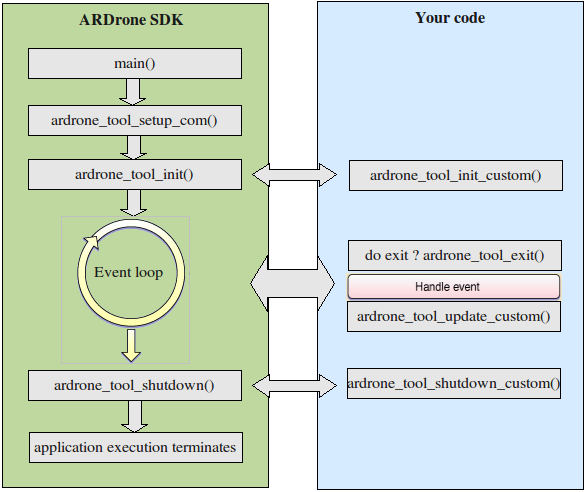
\includegraphics[scale=0.6]{mainloop.png}
    \caption{The application life cycle (picture from \href{https://projects.ardrone.org/embedded/ardrone-api/index.html}{\Ardrone API Webpage})}
    \label{mainloop}
\end{figure}

\subsection{Extending C With Python}
After we were able to safe an image frame to a file in C we could have Python read the file, process it, and send movements commands back to C. The main functions 
that took care of the initiation, updating and closing of the application instantiated and closed Python as well as updated Python. When C updated Python it supplied
Python with a tuple consisting of the frame counter (to retrieve the frame image) and the navigation data, and Python returned pitch, yaw, roll and gaz values (or something
to indicate that the application should exit). \\

While one might think that we decided to stick with the slowest manner to send the frame data from C to Python, it is not as bad as one would expect. Because each frame is
saved we could playback a run in which we flew with the \Ardrone and debug it completely and accurately. Later, we even saved the navigation data so we would be able to 
get an identical, simulated stream of information that was not actually send by the drone but rather read from file. This allowed us to easily debug any run and test 
probable solutions without flying with the \Ardrone over and over again. \\

Another something special we did with Python was using OpenCV. OpenCv can be used with Python quite easily, albeit some basic functions did not work even though everything
indicated it should be working, we were quite happy with it. \\

While it was not part of our direct goals, the bridge from the SDK written in C to our code written in Python using only one function that transfer all the necessary
data is something we expect could prove to be quite useful to other people as well. 




























\section{Methods Used}
We divided the first subtask in three subgoals: Finding the object; tracking the object and picking up the object. 

\subsection{Finding The Object}
To find the object we used a simple routine, in combination with a more complicated recognition. The routine is: Start flying at a low height, and then turn 360 degrees.
 While turning we constantly check the front camera (since we can only check one camera properly at the same time) for our object. If we had no indication of the object
at this particular height we would increase the search height and begin again. If the object had been found we would store that height and go back to that height when 
it was lost. This, in order to speed up the search process later on (it was not unknown for the \Ardrone to lose the object some times). \\

We chose to make an object that had a bright pink color. This simplified things for us: We only had to recognize a big enough surface of our color. We tried a couple of things to recognize our color:

The first step was to define the values that our color ranged from. We chose to divide our image in HSV values. This divides the image in 3 different layers: Hue, Saturation and Value. These layers represent the values of the image's ``Hue, Saturation and Value'' as shown in figure \ref{HSV}. OpenCV changes these values to a range of 0 to 255 (to create images it can show) by dividing the Hue by 2, and the saturation and value by $\frac{100}{255}$. The advantage of HSV above RGB (Red Green Blue) values is that it is easier to recognize of your color needs to be a bit lighter (thus, increasing the Value) than that your color needs to be a bit greener.

\begin{figure}
  \centering
      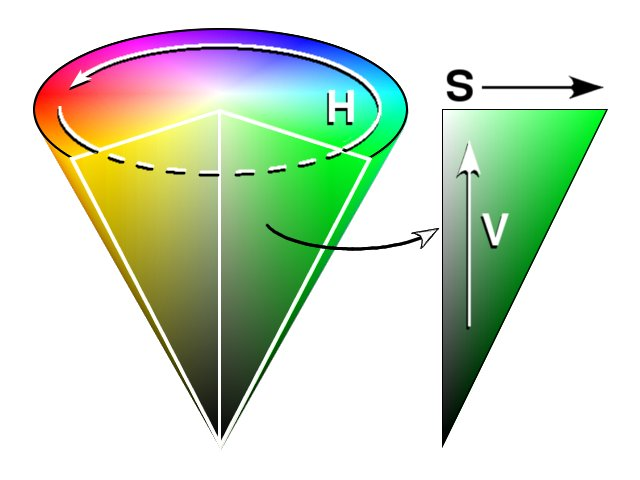
\includegraphics[scale=0.35]{HSV.jpg}
  \caption{Hue (H), ranging from 0 to 360 degrees; Saturation (S), ranging from 0 to 100\% and Value (V) ranging from 0 to 100\% }
  \label{HSV}
\end{figure}

OpenCV placed the pixels that were in the right HSV range in a new picture. This picture had a value of 1 on the pixel where our color-values were good, and a value of 0 where they were bad. This resulted in a white blob where almost every white pixel was on our object. Something like figure \ref{processed}. Unfortunately the computer can not understand this. We still need to let the \Ardrone know where the object is in this picture. To find the centre of the object, we tried histogram backprojection.

\begin{comment}% persoonlijk vind ik dit mooier maar hij moet wel een wit randje ertussen bouwen 
\begin{figure}
  \centering
  \subfloat[The image after the first processing.]{\label{fig:processed}
\includegraphics[width=2.1in]{processedImage}}
  \subfloat[The image after the second processing.]{\label{fig:processed2}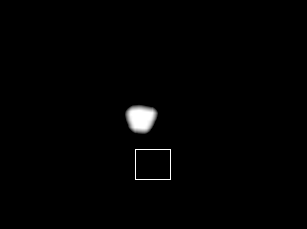
\includegraphics[width=2.1in]{processedImage2}}
  \caption{Results of processing a frame, the square in the right image debug-output.}
  \label{processed}
\end{figure}
\end{comment}

%\begin{comment} 
\begin{figure}
  \centering$
  \begin{array}{cc}
      
\includegraphics[width=2.5in]{processedImage.png} &
      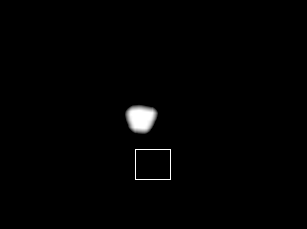
\includegraphics[width=2.5in]{processedImage2.png}
  \end{array}$
  \caption{Left: An example of our image after the first processing. Right: After the second processing. The square is just debug output.}
  \label{processed}
\end{figure}
%\end{comment}

\subsection{Tracking The Object}
Histogram backprojection is a technique that takes a histogram (a representation of the distribution of the colors in an image) of your target, and matches it for the
histogram of the same size of a part of the image around each position (x, y) in the image. Where the histogram of the target matches the histogram of some location in the
image a great deal, the location will have a big number. And, of course, it is the other way around for those locations that do not match. 
Unfortunately we experienced our first real problem with OpenCV, the function had a bug that we could never solve.  \\

Therefore we tried a different, somewhat simpler method, called ``Template Matching''. This is a bit like histogram backprojection, but instead of using histograms, we 
use a template of the object we wanted to see. This is is a somewhat less complicated method and it works a little bit less well but it did the trick. And 
since we allready had an image that was only black or white (0 or 1), our template simply had to be a white square. This would match the white space in our image, but not a
 single white pixel. This resulted in an image like in figure \ref{processed}. As you can see, the edges are a bit fuzzy. Now we can use the OpenCV function ``minMaxLoc'' 
to locate the centre of the object, which is the brightest pixel in the image. 
% we zouden hier nog de mooie formule van de opencv api in kunnen stoppen: 
% http://opencv.willowgarage.com/documentation/python/object_detection.html?highlight=template%20match

At first the size of our template was fixed. It was a 10 by 10 pixels square. This resulted in our second image having too many pixels with a value of 1 (and thus being the brightest). When we were able to calculate the distance of the object (see section \ref{sec:pickingUp}), we made the template size variable, meaning that we always exactly found the centre of the object. 

\subsection{Picking Up The Object}
We chose an object with a handle, and a hook on our \Ardrone. The advantage of this is that we do not have to hover above, or land on our object, but we can simply fly over it, and pick it up with the hook. This is a lot easier, because the \Ardrone has a flying error, which complicates hovering above the object. 

To be able to pick up the object we went through this routine:
\begin{itemize}
\item Put the centre of the object in a specified square (the white square in figure \ref{processed}). 
\item keep it there for a second, to compensate the flying error.
\item fly towards the target, while keeping it in the square
\item When the \Ardrone is close enough, switch to watching the bottom camera, fly a bit higher and fly forward, to pick up the object.
\end{itemize}
To be able to do these things, we had to do some tricky things:

\subsubsection{Calculate Distance}
The most important thing we did was calculating the distance to the object. The ammount of pixels that belong to our 
object should have some relation to the distance to the object because the object is smaller if we are further away
from it. So all We had to do was to count the number of non-zero pixels in the second processed
window. 
We calibrated this by counting the amount of those pixels for a number of known distances and
then used an online formula finder \footnote{\href{http://zunzun.com/FunctionFinder/2/}{Zunzun.com function finder}} to find the formula 
that calculates the distance. See equation \ref{eq:distanceFormula}.

\begin{comment}
     # coefficients
       a = 7.6315999175901217E-01
       b = -6.4523069253280248E-04
       c = 8.3189620080930808E+01
       d = -1.5517143254934185E-01
       f = 1.4487053946697799E+00
       g = -4.6478934298555246E-03
       Offset = 2.1482272389707244E-01

       temp = a * math.exp(b*x_in) + c * math.exp(d*x_in) + f * math.exp(g*x_in)
       temp = temp + Offset
       return temp
\end{comment}

\begin{equation}
willen we deze formule er ECHT in hebben?
\label{eq:distanceFormula}
\end{equation}

\subsubsection{Variable Steering Commands}
Another important factor in moving towards the object were variable steering commands. 
It is really important to steer towards the object quickly once you can. The faster the 
better because the flying errors are quite enormous. It is not unusual to see the \Ardrone
drifting off quite a bit even if we only want to rotate it 360 degrees. However, once
the \Ardrone has positioned itself in front of the object it will overshoot with the
corrections if it drifts of. To compensate for this effect we made sure the strength
of the steering values are lower as the \Ardrone is closer towards the target. This
is the case for pitch, yaw, roll and even the gaz commands. 

\subsubsection{Blind Flight}
The \Ardrone can only send one of the two video-streams over the network to our application. 
When we decide it is time to fly over the object, to pick it up, we switch to the bottom 
camera. This allows us to steer the \Ardrone in the right direction when we notice it drifting
off but in the mean time we do not see any of the more interesting data (the front view). If
we miss the object completely we might fly against a wall. To solve this we granted the
\Ardrone a limited amount of time on the bottom camera to pick up the object before we switch
back to the front camera and restore whatever it might have done. 

\label{sec:pickingUp}



























% In the presentation we had sections for problems and results, but I guess 
% we should just put that stuff in the other chapters (and as Arnoud said
% make it more like "we tried this and this but discarded that because that 
% and that)


\section{Results}

\section{Future Work}

\end{document}































